\documentclass[a4paper, 12pt]{article}

\usepackage[portuges]{babel}
\usepackage[utf8]{inputenc}
\usepackage{amsmath}
\usepackage{indentfirst}
\usepackage{graphicx}
\usepackage{multicol,lipsum}

\usepackage[hidelinks]{hyperref}   % adiciona links na TOC e nas citações

% Renomeia o título da TOC
\addto\captionsportuges{
  \renewcommand{\contentsname}
    {Sumário}
}

%%%%%%%%%%%%%%%%%%%%%%%%%%%%%%%%%%%%%%%%%%%%%%%%%%%%%%%%%%
% INÍCIO DO DOCUMENTO
%%%%%%%%%%%%%%%%%%%%%%%%%%%%%%%%%%%%%%%%%%%%%%%%%%%%%%%%%%

\begin{document}
%\maketitle

%%%%%%%%%%%%%%%%%%%%%%%%%%%%%%%%%%%%%%%%%%%%%%%%%%%%%%%%%%%
% CAPA
%%%%%%%%%%%%%%%%%%%%%%%%%%%%%%%%%%%%%%%%%%%%%%%%%%%%%%%%%%%
\begin{titlepage}
	\begin{center}
    	\begin{figure}[!ht]
        	\centering
        	
\includegraphics[width=3cm]{./imgs/uffs.png}
    	\end{figure}
    
    	\Huge{Universidade Federal da Fronteira Sul}\\
    	\large{Campus Chapecó}\\ 
    	\large{Bacharelado em Ciência da Computação}\\ 
    	
    	\vspace{15pt}
        \vspace{95pt}
        
        \textbf{\LARGE{Exercícios indicados nas aulas 05 e 06}}\\
    	
        \vspace{3,5cm}
	\end{center}
	
	\begin{flushleft}
	    \begin{tabbing}
			\textbf{Aluno:} Jean Carlo Hilger \\
			\textbf{Professor:} Andrei de Almeida Sampaio Braga \\
        \end{tabbing}
    \end{flushleft}
	
	\vspace{1cm}
	
	\begin{center}
		\vspace{\fill}
		Chapecó, março\\
		2021
	\end{center}
\end{titlepage}


%%%%%%%%%%%%%%%%%%%%%%%%%%%%%%%%%%%%%%%%%%%%%%%%%%%%%%%%%%%
% SUMÁRIO
%%%%%%%%%%%%%%%%%%%%%%%%%%%%%%%%%%%%%%%%%%%%%%%%%%%%%%%%%%%
\newpage
\tableofcontents
\thispagestyle{empty}

\newpage
\pagenumbering{arabic}

%%%%%%%%%%%%%%%%%%%%%%%%%%%%%%%%%%%%%%%%%%%%%%%%%%%%%%%%%%%
% Exercício 1
%%%%%%%%%%%%%%%%%%%%%%%%%%%%%%%%%%%%%%%%%%%%%%%%%%%%%%%%%%%
\newpage
\section{Exercício 1}

Construa um diagrama de estados com 3 estados para um autômato finito
não-determinístico que reconheça a linguagem $\{ w | w \text{ é uma string de }0\text{’s e }1\text{’s
que termina com }00\}$.

\subsection{Solução}

\begin{figure}[!ht]
    \centering
    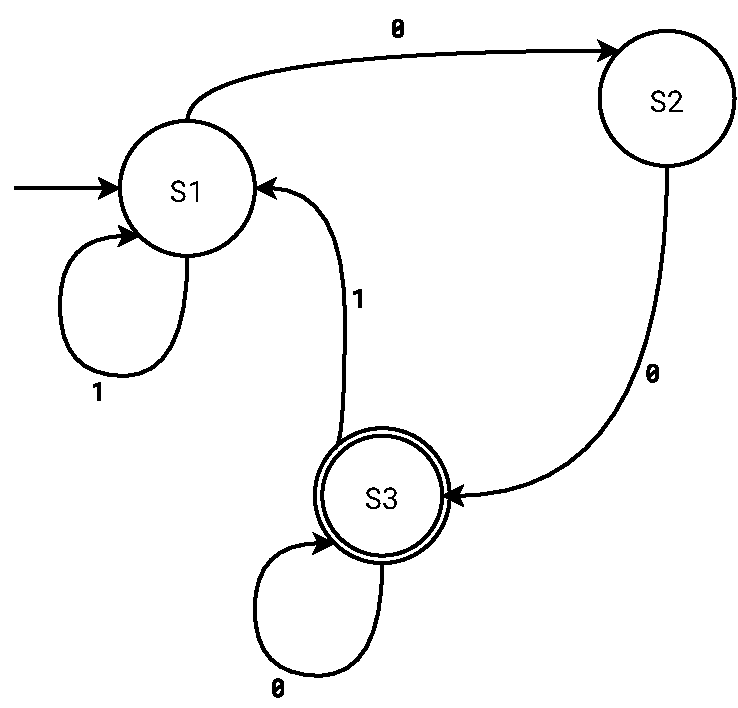
\includegraphics[width=6cm]{./imgs/task-2-1.pdf}
    \caption{Autômato não-determinístico solução}
    \label{fig:solution_t2_1}
\end{figure}


%%%%%%%%%%%%%%%%%%%%%%%%%%%%%%%%%%%%%%%%%%%%%%%%%%%%%%%%%%%
% Exercício 2
%%%%%%%%%%%%%%%%%%%%%%%%%%%%%%%%%%%%%%%%%%%%%%%%%%%%%%%%%%%
\newpage
\section{Exercício 2}
Descreva um autômato finito não-determinístico que reconheça a linguagem
que consiste de toda string do alfabeto $\{0, 1, …, 9\}$ tal que o último dígito da
string aparece antes na string.

\subsection{Solução}

Inicialmente, imaginemos o mesmo autômato para um alfabeto mais simples, formado apenas por $\{a, b\}$


\end{document}
